% !TEX encoding = UTF-8 Unicode
% !TEX spellcheck = en-US


% This is the root file of your thesis: thesis.tex
% A line starting with % is a comment. In some cases, I have included a command preceded by a %. You may activate the command by removing the %.

%%===================================
\documentclass[b5paper,twoside]{memoir}
\usepackage{ramsstyle}
\setstocksize{270mm}{175mm}

%%===================================
%Write the various parts of your thesis as separate files and include them into the main file by the command \include{name of included file}. When you compile the LaTeX file, you may choose which subfiles to include by the command

%\includeonly{chapter01,chapter02}

%%===================================
\begin{document}
\newcommand*{\fancyreflstlabelprefix}{lst}

\fancyrefaddcaptions{english}{%
  \providecommand*{\freflstname}{listing}%
  \providecommand*{\Freflstname}{Listing}%
}

\frefformat{plain}{\fancyreflstlabelprefix}{\freflstname\fancyrefdefaultspacing#1}
\Frefformat{plain}{\fancyreflstlabelprefix}{\Freflstname\fancyrefdefaultspacing#1}

\frefformat{vario}{\fancyreflstlabelprefix}{%
  \freflstname\fancyrefdefaultspacing#1#3%
}
\Frefformat{vario}{\fancyreflstlabelprefix}{%
  \Freflstname\fancyrefdefaultspacing#1#3%
}

% !TEX encoding = UTF-8 Unicode
%!TEX root = thesis.tex
% !TEX spellcheck = en-US

%This is the Titlepage
%%=========================================
\thispagestyle{empty}
%\includegraphics[scale=1.1]{fig/rams}
\mbox{}\\[6pc]
\begin{center}
\Huge{Power saving in high-level programming languages on embedded devices}\\[2pc]

\Large{Péter Henrik Haldorsen Gombos}\\[1pc]
\large{2015}\\[2pc]

PROJECT / MASTER THESIS\\
Department of Computer and Information Science\\
Norwegian University of Science and Technology
\end{center}
\vfill

\noindent Supervisor 1: Associate Professor Gunnar Tufte 

%\noindent Supervisor 2: Professor Fingal Olsson

 % This is the titlepage
\setcounter{page}{0}
\pagenumbering{roman}
% !TEX encoding = UTF-8 Unicode
%!TEX root = thesis.tex
% !TEX spellcheck = en-US
%%=========================================
\addcontentsline{toc}{section}{Preface}
\section*{Preface}
%Here, you give a brief introduction to your work. What it is (e.g., a Master's thesis in RAMS at NTNU as part of the study program xxx and\ldots), when it was carried out (e.g., during the autumn semester of 2021). If the project has been carried out for a company, you should mention this and also describe the cooperation with the company. You may also describe how the idea to the project was brought up.

%You should also specify the assumed background of the readers of this report (who are you writing for).\\[2cm]

\begin{center}
Trondheim, 2012-12-16\\[1pc]
(Your signature)\\[1pc]
Ola Nordmann
\end{center}
% !TEX encoding = UTF-8 Unicode
%!TEX root = thesis.tex
% !TEX spellcheck = en-US
%%=========================================
\addcontentsline{toc}{section}{Acknowledgment}
\section*{Acknowledgment}
I would like to thank the following persons for their great help during \ldots

If the project has been carried out in cooperation with an external partner (e.g., a company), you should acknowledge the contribution and give thanks to the involved persons.

You should also acknowledge the contributions made by your supervisor(s).

\begin{flushright}
O.N.\\[1pc]
(Your initials)
\end{flushright}
% !TEX encoding = UTF-8 Unicode
%!TEX root = thesis.tex
% !TEX spellcheck = en-US
%%=========================================
\addcontentsline{toc}{section}{Summary and Conclusions}
\section*{Summary and Conclusions}
Here you give a summary of your your work and your results. This is like a management summary and should be written in a clear and easy language, without many difficult terms and without abbreviations. Everything you present here must be treated in more detail in the main report. You should not give any references to the report in the summary -- just explain what you have done and what you have found out. The Summary and Conclusions should be no more than two pages.

You may assume that you have got three minutes to present to the Rector of NTNU  what you have done and what you have found out as part of your thesis. (He is an intelligent person, but does not know much about your field of expertise.)
% !TEX encoding = UTF-8 Unicode
%!TEX root = thesis.tex
% !TEX spellcheck = nb-NO
%%=========================================
\section*{Sammendrag}
Test
Dette er en test.

\tableofcontents
\setcounter{page}{0}
\pagenumbering{arabic}
% !TEX encoding = UTF-8 Unicode
%!TEX root = thesis.tex
% !TEX spellcheck = en-US
%%=========================================
\chapter{Introduction}
An embedded system is a computer system which is embedded in the devices it controls, and is designed for a dedicated usage.
Some examples of systems dedicated to a specific purpose are mobile phones, sensors and ATMs.
By embedding a computer system, the hardware can be specifically tailored for the application of the system.
The application of the system also adds constraints, and the solutions may contradict other constraints
In a battery driven system, a really powerful battery that lasts a long time would be better, but the size of the battery might make it no longer suitable for using the system on the move.
\todo{Find a big ass battery}
Other constraints that are often imposed on the systems are memory size, storage space, maximum operating temperature and physical size. (\cite{computercomponents} \cite{embeddsystems}

Power constraints are one of the most prevalent in current embedded systems, as more and more devices are connected to the Internet, and regular needs charging.
But some systems can’t be charged at regular intervals, for example sensor systems in areas that are hard to reach, on the bottom of the sea, embedded in concrete or someplace else; need to be able to function for a long time on a single battery.
As lower energy use also means lower heat dissipation, better power usage will lead to a cooler system, which is very important in handheld devices like mobile phones. 

In the early days of computing\todo{edit cliche}, the way the computers were programmed was with binary code, which is tedious to write, and requires the programmer to remember various arbitrary codes. 
Quite early\todo{when}, assembly languages were developed, which provides a one-to-one mapping of easier to remember function names to the machine code.
While far better for the programmer, assembly programming is still very time consuming and difficult to write, and when creating a big complex language, the data models the assembler provides are too basic. 
Virtually all programs written today are written in a high-level programming language, which means they are not a direct mapping of machine functions, but code written in it need to be transformed into something the machine can run. 
This transformation can happen in two different ways, compilation or interpretation. 

A compiler is a program that takes source code in a given language as input, and outputs code in some other form. 
This can either be into a lower level language, like assembly, or into another programming language entirely.
This source-to-source compiling is also known as transcompiling, or simply transpiling.
The compiled program when run takes the input and produces an output. 
An interpreter, on the other hand, is a program running the code, and takes the input at the same time and produces the output.
\missingfigure{Overview of compiler and interpreter }

While compilation and interpretation give a lot of advantages, they do add some overhead while running programs. 
A perfect compilation\todo{some other term} will translate the source code into an equivalent with no more instructions than needed, which is impossible except in trivial cases, as high-level languages adds many abstractions that are not easily translated to the basic data models of assembly languages. 
In the case of interpretation, the interpreter running on the computer by definition adds extra instructions. 
\todo{Remove however}However, the computer can do things to the source code that are not natural for a programmer, like statistical analysis, which can lead to other optimizations like dead code elimination, loop unrolling etc.\todo{What are these? Some other place}

JavaScript is a dynamic, weakly typed language, originally created for allowing interactivity on web pages.
Developed in 1995 by Netscape, it became the basis of the ECMAscript standard in 1997. (\cite{jshistory})
This standardization of JavaScript to work in every browser allowed it to become the most used programming language on the web.
Currently, almost 90\% of web pages uses JavaScript (\cite{jsclientstats}).
Newer developments in the JavaScript world is the node.js, later forked into io.js, a stand alone framework for running the V8 engine, allowing for the use of JavaScript on the server side.
In just three years, JavaScript is now used on 0.2\% of websites for server side code.(\cite{jsserverstats})

This dominance of JavaScript on the web has created to a large community around the language, with a lot of tools .\todo{show community - npm?}
For some, there is a want to use one language to do everything, and so multiple projects for using JavaScript on embedded platforms have risen.\todo{"For some, there is a want" - bad sentence}
In addition to the benefits of a high-level language, there is the added bonus of not having to use time to learn a new programming language when developing for an embedded platform.



\section{Related work}
The first look at how you can optimize software to achieve better energy performance was done by \cite{tiwari94}.
Before their work, power measurement tools where only available at the circuit and logic level.
They then introduce a way of estimating the energy cost of the instructions that are available on the processor, by measuring the current into the microprocessor with an ammeter, and a model for estimating the power consumption of a program by looking at the instructions of the program.
With these data, they can optimize code running on the processor by using a strategy that minimizes the use of power hungry instructions.

In \cite{russell98}, finds that the model developed by \cite{tiwari94} is needlessly detailed, and that the power consumption of a program can be estimated within 8\% accuracy by using the average power consumption per cycle of the processor, multiplied with the execution time in cycles of the program.
Their conclusion then is that to optimizations that minimize execution time of a program, also reduces the energy consumption of the same program.

\cite{ortiz08} looked at some source code optimizations to find if they would lower the energy consumption, but found that the impact of the techniques varied on the platforms they tested against.
This device specific optimization was explored further by \cite{delima13}, where the authors try to find a set of compiler optimizations that gives the best result for the program.
They do this by reducing the number of possible sets of optimizations and test code compiled with the sets of optimizations, finding the set that provides the best performance gain or is most power efficient.
While their research focuses on a desktop computer, the same could be done for an embedded system.

\todo{Write about Kavvadias}
\todo{More literature}

\section{Problem}
To create embedded systems, there’s often a need to use lower level languages, to 
achieve the desired power and speed requirements.
It can be quite hard to program in these languages, with few abstractions and a need for the programmer to do a lot of dirty work.
On the other hand, high-level languages offer many improvements for the programmer, as well as a familiar programming environment.
Unfortunately, high-level language often mean a high level of energy use.
To consolidate these directions, this thesis ask the question: “What are energy efficient ways of bringing high-level programming languages to embedded devices?”

This will be explored through comparing the energy use of some JavaScript engines, particularly with the Tessel 1, and a Raspberry Pi board running Espruino and io.js, while running benchmark code.

\section{Outline of this thesis}
In chapter \ref{ch:chapter2} the method of the experiment is explained, together with the rationale behind the experiment.
The results of the this experiment is presented in chapter \ref{ch:chapter3}, and these are discussed in chapter \ref{ch:chapter4}.
Concluding remarks are added in chapter \ref{ch:chapter5}.
% !TEX encoding = UTF-8 Unicode
%!TEX root = thesis.tex
% !TEX spellcheck = en-US
%%=========================================
\chapter{Energy Efficiency, Hardware and Software View}
\label{ch:chapter2}

To create an energy efficient computer, there are two main parts 

\section{Hardware}
Optimized hardware

Multi-cores heterogenous - cite SHMAC

\section{Software}
Optimizations \todo{examples}
Sleeping
% !TEX encoding = UTF-8 Unicode
%!TEX root = thesis.tex
% !TEX spellcheck = en-US
%%=========================================
\chapter{Method}
\label{ch:chapter3}


To fulfill the goal of this thesis, an experiment to compare the energy use of different JavaScript engines was developed.
Using a independent power supply, giving a stable voltage, and then measure the current drawn from the hardware platforms while executing programs run in a JavaScript engine.
These measurements can be used to find the power used by a single program, and by running the program a large number of times, an average power consumption of the program can be obtained.
All of the programs are trivial operations in a loop, and using the average consumption, the energy cost of a single expression in the JavaScript engine can be found.

The goal of the experiment is to look at differences in the energy use of the different JavaScript implementations, which means that it is not the exact numbers that are of interest, but rather the trends that the numbers show.
For the experiment, this translates to being approximate whenever it is appropriate.


\subsection{Programs}
Four programs were used on each tested platform, all following a similar pattern: In a loop repeated 1,000,000 times, some expression is evaluated.
The programs are named  are addition, multiplication, closure and bit shift; testing various JavaScript features.
The addition program can be seen in \fref{lst:add}


\begin{lstlisting}[language=JavaScript,caption={Addition program}, label={lst:add}]
for(var i = 0; i < 1000000; i++) {
        var a = 1;
        var b = 2;
        var c = a + b;
}
\end{lstlisting}

\todo{Talk about the program - might be in discussion too}

%http://git-public.pengutronix.de/?p=OSELAS.BSP-EnergyMicro-Gecko.git;a=summary

\section{Hardware Platforms}

\begin{table}[h]
\centering
\begin{tabular}{| c | c | c |}
\hline
            & Raspberry Pi  & Tessel        \\ \hline
CPU         & BCM2835       & LPC1830       \\ \hline
Core        & ARM1173       & ARM Cortex M3 \\ \hline
Architecture& ARMv6         & ARMv7         \\ \hline
Clock Speed & 700 MHz       & 180 MHz       \\ \hline
RAM         & 512 MB        & 32 MB         \\ \hline
Flash       & SD-card       & 32 MB         \\
\hline
\end{tabular}
\caption{Comparing a Tessel 1 with a Raspberry Pi 1 Model B}
\label{tab:specs}
\end{table}


As can be gathered from \fref{tab:specs}, the Raspberry Pi is a much faster machine than the Tessel, clocked almost 4 times higher, and with 16 times the amount of RAM.
This means that the Raspberry Pi is able to run much bigger software and do it faster, but also that it will use a lot more power.

\subsection{Silicon Labs EFM32GG STK3700}

\section{Software Platforms}
\subsection{Tessel}
The goal of the Tessel\footnote{https://tessel.io} platform is to be an easy way of giving new developers access to hardware programming.

One of the rationales behind choosing Lua as the intermediate language (and the Tessel 1 way of running code on a microcontroller) was that Lua has a low memory profile and is generally embeddable.
At the time, the only choice in JavaScript engine was the V8 engine, and the goal for Tessel was to cater for low energy use.
The next step in this direction was to use LuaJIT to get a much more optimized running of programs.(\cite{newengine})

To be able to write JavaScript and run it as Lua, the JavaScript code needs to be translated.
In the Tessel stack, the Colony Compiler\footnote{https://github.com/tessel/colony-compiler} does this translation, using simple lexical parsing, i.e. changing JavaScript features directly into Lua equivalents.

Running now on the Tessel is the LuaJIT virtual machine, which is much faster than the standard Lua engine, due to a more efficient design. While there was a goal to enable the just-in-time compilation, the developers of Tessel has since decided that some of the goals of the project can’t be reconciled with a real low power usage, and the next version of Tessel will run node/io.js.(\cite{movingfaster})

\subsection{Espruino}
Espruino\footnote{http://www.espruino.com/} has, in addition to the goal of Tessel to bring hardware to new people, also the goal of doing it as efficient as possible.
The implementation is targeted to devices with memory as small as 128kB Flash and 8kB RAM, way less than both hardware platforms that are used in this experiment provides.
To achieve this goal, a number of trade-offs has been done to the implementation.

The Espruino VM is an almost complete JavaScript implementation, missing some elements due to the memory limits imposed by the design goal. 
Mainly, the big difference between Espruino and other JavaScript implementations, is that it does not translate the source code to byte code, but executes the source directly. 
This is again due to memory concerns, as the developers want the source code to be on the device when executing, to be able to edit the source code on the device. 
If the VM translated to byte code, it would need twice the storage for the same program to keep it all on the device.

Other optimizations done for memory minimization (and thus speed) include using a linked list for storage of arrays and objects (allowing for constant time insertion and deletion) and including typed arrays, which is a direct mapping of memory to the data structure.

While the platform itself is designed to be power efficient, it does not optimize the code before running it, requiring the programmer to write efficient code. 
Adding some middleware to optimize code before running it on the Espruino could help minimizing the energy use.

\todo{citations}

\subsection{io.js/node.js}
Node.js/io.js\footnote{https://iojs.org} is developed to run JavaScript on computers, using the V8 Engine, found in browsers such as Google Chrome.
As the normal running environments for Node are not restricted on energy, the platform is optimized for speed.
This does not mean that the platform is power hungry, as speed optimizations might lead to better energy efficiency as well.
In fact, Technical Machine has announced that they will use io.js for the Tessel 2, that will release in the fall of 2015.(\cite{movingfaster})

In this experiment, the Node.js fork io.js will be used, as it is currently more updated than Node.js.
The io.js team has recently announced that they will be joining the new Node Foundation, and the project that is currently io.js, will be renamed Node in the near future.
While this brings a bit of terminology problems in this thesis, when either io.js or Node.js is mentioned, it can be assumed that it is io.js that is used.


\subsection{Linux}
To run programs on the Raspberry Pi, an operating system is needed, 
The Raspbian OS, based on the Debian Linux distribution, 

Provided with the Raspberry Pi is the Raspbian OS, based on the Debian Linux distribution.

\todo{Write this}

% http://sjoerd.luon.net/posts/2015/02/debian-jessie-on-rpi2/



\section{Experimental setup}

\begin{figure}[ht]
\centering
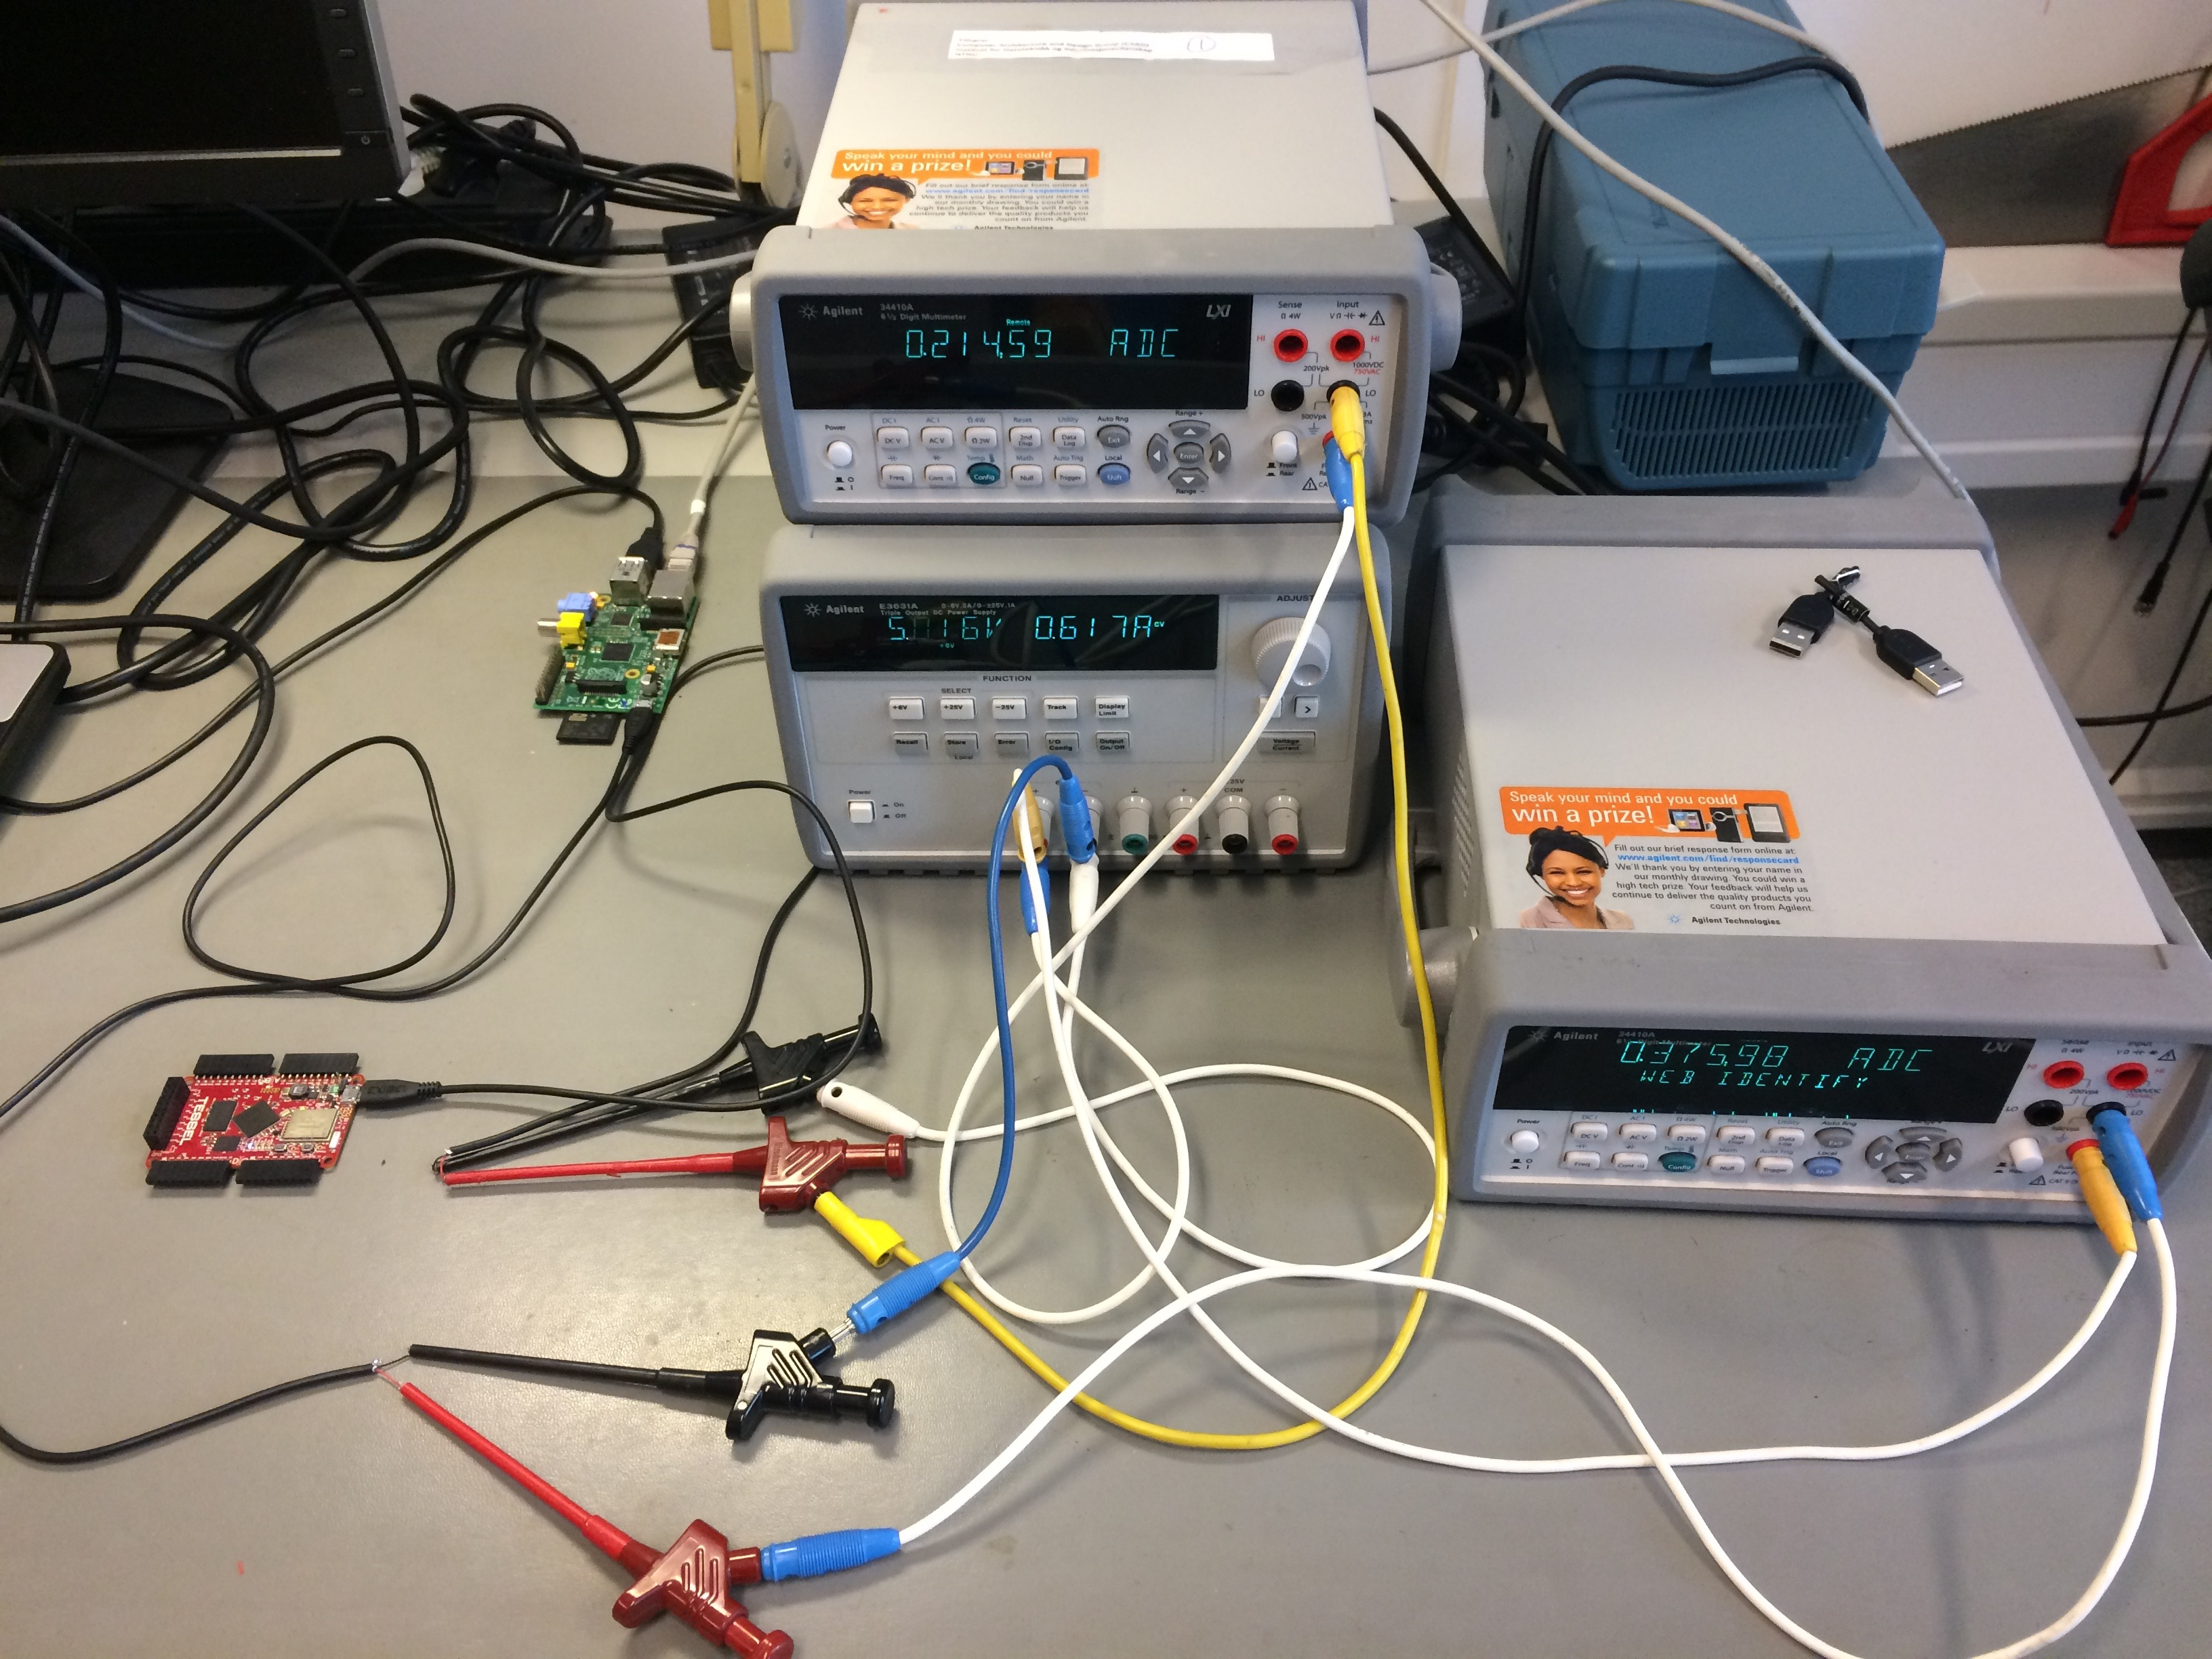
\includegraphics[width=\textwidth]{fig/pics/setup.jpg}
\caption{The hardware setup of the experiment}
\label{fig:setup}
\end{figure}

To power the experiment, the Agilent E3631A was used. 
As both the hardware platforms were running experiments at the same time, they were both connected to the power supply, with a common ground. 
The multimeter, Agilent 34410A, was connected in series between the power supply and the device, set to ADC measurement. 
There was one multimeter for each device while running in parallel.
Both devices receives power through a Micro USB cable.
A cable was cut up, and using clamps, the power and ground wires were connected to the power supply.(\cite{usbmicro})

The multimeter supports logging over LAN, allowing to remotely monitor the experiment.
Using the Keysight Benchvue Software, all measurements can be exported in CSV format.
Together with the Raspberry Pi's remote SSH-access, the experiments on the Pi can be remotely started and controlled.
To fully automate the experiment on the Raspberry Pi, a shell script was written to restart the program for as many times that was required in the experiment.
After each run, the device would sleep for 0.5 seconds before the reset, to differ between each run while running.

Unlike the Raspberry Pi, the Tessel hardware does not allow for remote access while it is running on external power, because the USB port is the only communication port able to flash the Tessel.
To work around this problem, the program was written to the internal flash, which will start to run whenever the Tessel boots.
Then the hardware was reset from software after each program run.
This feature did not exist in the platform, but was written for this experiment, and has since been accepted into the project.\footnote{\url{https://github.com/tessel/t1-firmware/pull/140}}
After approximately the wanted number of runs were done, the logging was stopped.

Another way of doing it could have been to create an USB cable with only data wires from a computer and connect those to the data wires on the cable going to the device. \todo{Should I mention this?}


\subsection{Data manipulation}
The Benchvue Software can export the measurement data in CSV format, in two columns with time stamp and the sampled data at that time stamp.
These files were read in a Python program, which did the manipulations needed on the data.

To find the average power consumption of every run on Raspberry Pi, the fact that the current drawn while it was sleeping was always under 0.39 m/micro A, and always above when the program was running, was exploited. 
Stripping away everything under this threshold, and splitting this stream up into blocks of as many samples as the average program contains, the energy consumed by each program in the run can be added up to. 
The average of these sums is then the average power usage of one experiment.

The Tessel data was not as easy to manipulate, as the board reset procedure is not as clear when it begins and ends from the current data. To get a similar data set to work on as from the Raspberry Pi, as many samples as go into the board reset is removed after the number of samples of the average program is removed.

\todo{On achieving the desired numbers}
% !TEX encoding = UTF-8 Unicode
%!TEX root = thesis.tex
% !TEX spellcheck = en-US
%%=========================================
\chapter{Results}
\label{chap:chapter4}
%Voltage running both Raspberry Pi and Tessel on: 5.015 V

In this chapter the results of all the experiments are presented.

Shown are the base power usage of both tested hardware platforms, i.e. the current drawn when no program is running.
This is done to see what amount of the current drawn when running the other experiments are due to the operation of the device.
The Raspberry Pi is shown to draw more than twice the current than the Tessel.

Next the approximate time for running the various programs on each software platform are tabulated.
These numbers are used to later find the average current drawn by a program run.

Then graphs of the current samples taken of each program on every platform are shown, to illustrate how a program run typically is.

In \fref{sec:avgcurrent}, the average current drawn per sample is shown, allowing for direct comparison with the results from \fref{sec:basepower}.
The results show that the Tessel draws far less current than the Raspberry Pi, but also that the Espruino VM draws less than io.js.
To explain this, the number of iterations per sample is shown in the section after, where it is shown that io.js manages to perform an order of magnitude more iterations per sample than the other platforms.

Lastly, the calculated average current drawn and power used by a single iteration in each program on every platform is shown.
Here it can be seen that despite drawing the most amount of current when running, io.js is the most efficient one per iteration.

\section{Base Power Usage}
\label{sec:basepower}
In figures \ref{fig:baserasp} and \ref{fig:basetessel}, power measurements of both hardware platforms running with no active program are graphed.
When the Raspberry Pi is running here, it is with a Linux distribution.
All the noise that can be seen is various background programs running, like networking and resource management.

With a sample set over 10 minutes, the average current drawn per sample is $0.378\si{\ampere}$ on the Raspberry Pi with no running program.

\begin{figure}[h!]
\centering
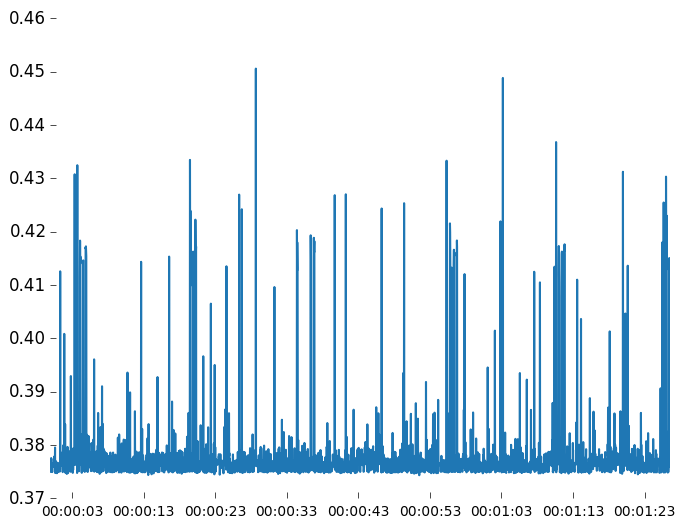
\includegraphics[scale=0.55]{fig/graphs/baseuse_rasp.png}
\caption{The Raspberry Pi running with no active program}
\label{fig:baserasp}
\end{figure}
\newpage

\begin{figure}[h!]
\centering
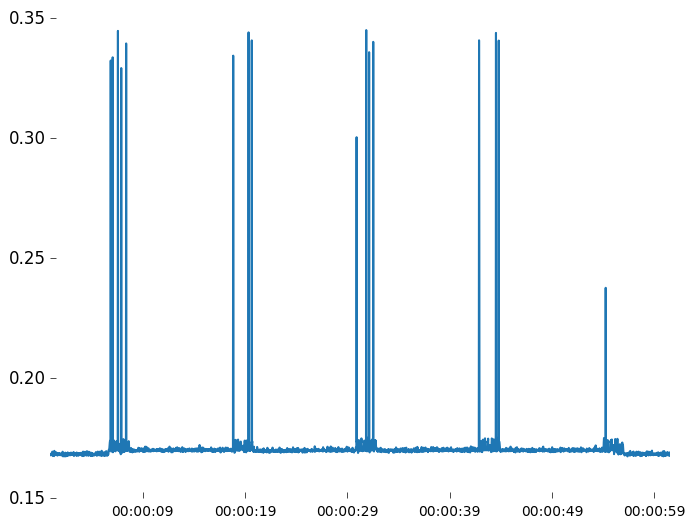
\includegraphics[scale=0.6]{fig/graphs/baseuse_tessel.png}
\caption{The Tessel running with no active program}
\label{fig:basetessel}
\end{figure}

In the Tessel graph, there is a lot less noise.
The high readings that can be seen, are from the WiFi-chip that is included.
About every 12 seconds, it checks the list it gathers of WiFi networks in range, to see if any of them are recognized.

With a sample set over 10 minutes, the average current drawn per sample is $0.162\si{\ampere}$ on the Tessel with no running program.

\section{Program time}
In \fref{tab:timedruns}, the approximate times of running the programs are gathered.
To note is the running time of the Left shift program on the Tessel, which is much higher than any other running time.
The closure program also systematically use longer time on every platform.
\begin{table}[h]
\centering
\begin{tabular}{ c  c  c  c  c }
 & Addition & Multiplication & Left shift & Closure \\ \midrule
 \rowcolor[gray]{.9}
 Espruino &  0m 48s & 0m 48s & 0m 49s & 1m 19s \\ 
 \rowcolor[gray]{.5}
 io.js  & 0m 3s & 0m 3s & 0m 3s & 0m 4s \\ 
 \rowcolor[gray]{.9}
 Tessel & 0m 19s & 0m 19s & 6m 12s & 2m 17s\\ 
 \bottomrule
\end{tabular}
\caption{Approximate time of each program}
\label{tab:timedruns}
\end{table}



\section{Current samples}
This section shows the results gathered by the multimeter, as described in \fref{sec:expsetup}.
The only manipulation done to this data is cutting it to not show the whole experiment, but rather just some interesting parts for illustration.

\begin{figure}[h!]
\centering
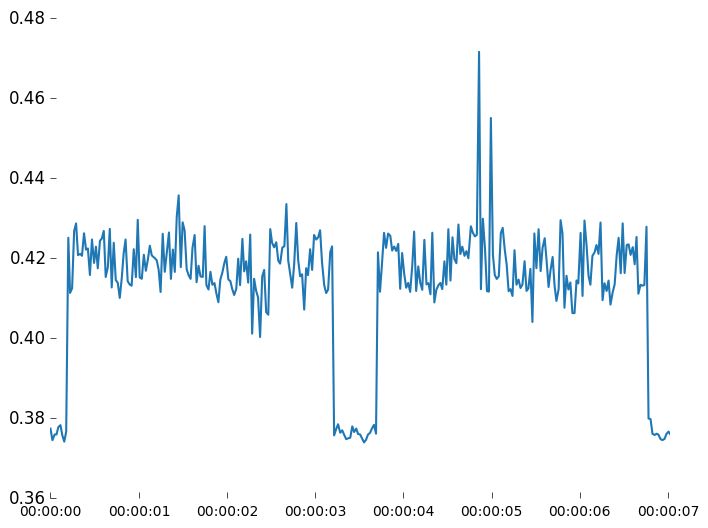
\includegraphics[scale=0.6]{fig/graphs/addition_iojs.png}
\caption{The addition program running in io.js on Raspberry Pi}
\label{fig:addraspio}
\end{figure}
\Fref{fig:addraspio} shows two complete runs of the addition program, which was shown in \fref{lst:add}, in io.js on the Raspberry Pi.
The dips in the readings are the sleep period between each run of the program.
As many parts of the OS is paused when the sleep command is issued, the spikes that could be seen in \fref{fig:baserasp} is not present between the program runs.


\begin{figure}[ht]
\centering
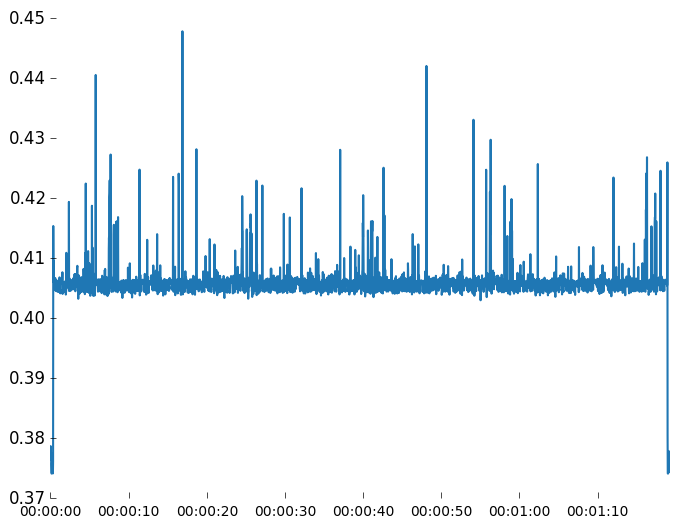
\includegraphics[scale=0.6]{fig/graphs/closure_espruino.png}
\caption{The closure program running in Espruino on Raspberry Pi}
\label{fig:closesp}
\end{figure}
Shown in \fref{fig:closesp}, is a single run of the closure program.
As the program running time is at about the same length as the run with no program shown in \fref{fig:baserasp}, the spikes here are similar to the graph when running with no program.
The dips, seen  are identical with \fref{fig:addraspio}

\clearpage

\begin{figure}[h!]
\centering
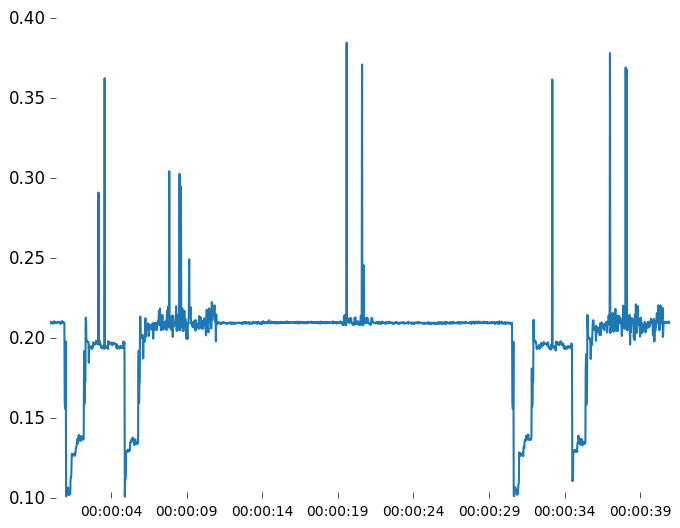
\includegraphics[scale=0.6]{fig/graphs/tessel_multi.png}
\caption{The multiplication program running on the Tessel 1}
\label{fig:multtes}
\end{figure}
In \fref{fig:multtes}, a single run of the multiplication program on the Tessel is shown, as well as the two power resets of the device on either side.
The WiFi chip turning on can also be seen in the middle of the graph.


\section{Average current drawn per sample}
\label{sec:avgcurrent}



\newcolumntype{A}{>{\columncolor[gray]{.9}}m{1.3cm}}
\newcolumntype{D}{>{\columncolor[gray]{.8}}m{1.3cm}}
\begin{table}[h!]
\centering
\begin{tabular}{c c}
    \begin{tabular}{c A}
    \multicolumn{2}{c}{Add}\\
    Espruino & 0.409 \si{\ampere} \\
    io.js & 0.419 \si{\ampere} \\
    Tessel & 0.203 \si{\ampere}
    \end{tabular} &
    
    \begin{tabular}{c A}
    \multicolumn{2}{c}{Multiplication} \\
    Espruino & 0.409 \si{\ampere}\\
    io.js & 0.419 \si{\ampere} \\
    Tessel & 0.203 \si{\ampere}
    \end{tabular} \\
& \\
    \begin{tabular}{c A}
    \multicolumn{2}{c}{Shift} \\
    Espruino & 0.409 \si{\ampere} \\
    io.js & 0.419 \si{\ampere} \\
    Tessel & 0.219 \si{\ampere}
    \end{tabular} &
    
    \begin{tabular}{c A}
    \multicolumn{2}{c}{Closure} \\
    Espruino & 0.406 \si{\ampere} \\
    io.js & 0.422 \si{\ampere} \\
    Tessel & 0.215 \si{\ampere}
    \end{tabular}
\end{tabular}
\caption{Average current drawn per sample}
\label{tab:avgcurrent}
\end{table}

\Fref{tab:avgcurrent} shows the average current drawn per sample of each program, with the same data as used in \fref{tab:results}.
As can be seen, io.js draws the most current per sample.

\section{Iterations per sample}
Using the number of samples taken in the experiments, the number of iterations is done per sample is shown in \fref{tab:iterpersample}.
These values are tied to how fast the programs run, as a program that runs for a longer time will be sampled more often, as the sample rate is constant.
\begin{table}[h!]
\centering
\begin{tabular}{c c}
\begin{tabular}{c A}
    \multicolumn{2}{c}{Add}\\
    Espruino & 4.8  \\
    io.js & 64.0 \\
    Tessel & 8.1
    \end{tabular} &
    
    \begin{tabular}{c A}
    \multicolumn{2}{c}{Multiplication} \\
    Espruino & 4.7\\
    io.js & 64.1\\
    Tessel & 7.8
    \end{tabular} \\
& \\
    \begin{tabular}{c A}
    \multicolumn{2}{c}{Shift} \\
    Espruino & 4.6 \\
    io.js & 63.9 \\
    Tessel & 0.7
    \end{tabular} &
    
    \begin{tabular}{c A}
    \multicolumn{2}{c}{Closure} \\
    Espruino & 3.0 \\
    io.js & 63.9 \\
    Tessel & 1.8
    \end{tabular}
\end{tabular}
\caption{Iterations per sample}
\label{tab:iterpersample}
\end{table}

\section{Energy use per iteration}

\newcolumntype{C}{>{\columncolor[gray]{.9}}m{1.3cm}}
\newcolumntype{D}{>{\columncolor[gray]{.8}}m{1.3cm}}
\begin{adjustwidth}{-1cm}{}
\begin{table}[ht]
\centering
\begin{tabular}{m{7cm} m{5cm} }
    \begin{tabular}{c C D C}
    & \multicolumn{3}{ c }{Add}  \\
    & Tessel & io.js & espruino  \\
    {\tiny Current (\si{\micro\ampere})} & 158.18 & 55.286 & 844.32  \\
    {\tiny Power (\si{\micro\watt})} & 793.27 & 277.26 & 4,234.3 \\
    \end{tabular} &

    \begin{tabular}{C D C}
    \multicolumn{3}{ c }{Multiplication} \\
    Tessel & io.js & espruino \\
    165.67 & 55.276 & 844.16 \\ 
    830.84 & 277.21 &  4,233.5 \\
    \end{tabular}\\

    & \\
    \begin{tabular}{c C D C}
    & \multicolumn{3}{ c }{Closure} \\
    & Tessel & io.js & espruino \\
    {\tiny Current (\si{\micro\ampere})} & 1,196.3 & 70.896 & 1347.9 \\
    {\tiny Power (\si{\micro\watt})} & 5,999.4 & 355.54 & 6,759.7
    \end{tabular} &
    
    \begin{tabular}{C D C}
    \multicolumn{3}{ c }{Shift} \\
    Tessel & io.js & espruino \\
    3,334.5 & 55.276 & 862.05 \\
    6,723 & 277.21 & 4,323.2
    \end{tabular}\\

\end{tabular}
\caption{Energy per iteration in loop}
\label{tab:results}
\end{table}
\end{adjustwidth}

In \fref{tab:results}, the calculated average current drawn and power used per iteration in each program is collected.
The values are shown in \si{\micro\ampere}, but as the number of iterations is 1,000,000, the values in the table is also representing the current drawn for the entire program run.

% !TEX encoding = UTF-8 Unicode
%!TEX root = thesis.tex
% !TEX spellcheck = en-US
%%=========================================
\chapter{Conclusion}

% Include more chapters as required.
%%=========================================
%\appendix
%% !TEX encoding = UTF-8 Unicode
%!TEX root = thesis.tex
% !TEX spellcheck = en-US
%%=========================================

\chapter{Acronyms}
\begin{description}
\item[FTA] Fault tree analysis
\item[MTTF] Mean time to failure
\item[RAMS] Reliability, availability, maintainability, and safety
\end{description}
%% !TEX encoding = UTF-8 Unicode
%!TEX root = thesis.tex
% !TEX spellcheck = en-US
%%=========================================

\chapter{Additional Information}
This is an example of an Appendix. You can write an Appendix in the same way as a chapter, with sections, subsections, and so on.

%%=========================================
\section{Introduction}

%%=========================================
\subsection{More Details}
% Include more appendices as required.
%%=========================================
\bibliographystyle{apa}
%\addcontentsline{toc}{chapter}{\bibname}
\bibliography{refs}  
%%=========================================
%%% !TEX encoding = UTF-8 Unicode
%!TEX root = thesis.tex
% !TEX spellcheck = en-US

%This is the Curriculum Vitae
%%=========================================
\addcontentsline{toc}{chapter}{Curriculum Vitae}
\chapter*{Curriculum Vitae}
\hrule
\begin{minipage}[t]{0.65\linewidth}
\begin{tabular}{ll}
Name: & \textbf{Your Name}\\
Gender: & Female\\
Date of birth: & 1. January 1995\\
Address: & Nordre gate 1, N--7005 Trondheim \\
Home address: & King's road 1, 4590 Vladivostok, Senegal\\
Nationality:    & English \\
Email (1): & your.name@stud.ntnu.no\\
Email (2): & yourname@gmail.com\\
Telephone: & +47 12345678\\
\end{tabular} 
\end{minipage}\hfill
\begin{minipage}[t]{0.25\linewidth}

\includegraphics[scale=0.3]{fig/me}\\[1pc] Your picture
\end{minipage}
\hrule

%%=========================================
\section*{Language Skills}
Describe which languages you speak and/or write. Specify your skills in each language.

%%=========================================
\section*{Education}
\begin{itemize}
\item School 1
\item School 2
\item School 3
\end{itemize}

%%=========================================
\section*{Computer Skills}
\begin{itemize}
\item Program 1
\item Program 2
\item Program 3
\end{itemize}

%%=========================================
\section*{Experience}
\begin{itemize}
\item Job 1
\item Job 2
\item Job 3
\end{itemize}

%%=========================================
\section*{Hobbies and Other Activities}         % Your curriculum Vitae     
%%=============================================

\nocite{*}
\end{document}
